\section{总体设计}
\subsection{新的编程模型}
基于produce-consume模型,以及隔离的地址空间的需求,
我们不再使用pthread实现SMR,而是重新实现了一个线程模型。
这个线程模型与传统的pthread线程不同:
(1)其中每个线程都拥有自己独立的地址空间,
线程之间相互隔离,不需要共享主进程的地址空间;
(2)线程之间有一个共享的channel,
用于线程间的通信。
每个map worker和reduce worker就是这样一个线程,
并且我们在初始化的时候,
让每个map worker和reduce worker之间拥有一个共享的channel,
用于传递map产生的中间结果。

\subsubsection{Phoenix较差scalability的分析}
必须结合应用程序的特点来说明问题:
\redt{是什么导致speedup下降(pagefault),为什么hist, wc, sm的pagefault会比较多,为什么pca, sm的pagefault会比较少?}
我们能够做的改进是不是只对那种pagefault比较读的应用程序有效果呢?
\subsubsection{线程模型}
Linux操作系统中,使用一个lock来保护地址空间的目的是……

为了避免produce-consumer模型如图
每个map线程的地址空间中有


%多个worker之间,地址空间隔离,从而不会产生过多的spinlock.
如图\ref{phoenix:speedup}的数据显示,
8核以上,Phoenix处理相同数据集的时间时间越来越长。
我们试图通过性能工具Perf\cite{},
深入分析影响scalability的主要原因。
Perf的实验结果显示,16核与32核情况下,
hist中占用时间最多的函数是ticket\_spin\_lock,
分别为40.5\%和71.25\%,即应用程序运行中的绝大部分的时间用于spinlock,
而未做时间的运算。
通过分析perf record记录的函数调用栈,
我们发现ticket\_spin\_lock是源于page-fault。
内核中page-fault函数需要操作raw\_spin\_lock,
该spin\_lock是产生ticket\_spin\_lock的主要原因。

由于Phoenix采用Pthread线程模型,
多个线程之间需要共享很多内核态数据结构,
特别地,当多个线程并发执行时,
会引起很多的page-faults。
Linux内核源码显示,
当发生page-faults时,线程首先需要获取进程的mm\_sem信号量
——该信号量属于一个进程私有的信号量,用于保护进程的映射表,
以及pagetable\_lock用于保护一个进程的页表。
当进程的多个线程并发的访问mm\_sme信号量时,
将会导致线程对信号量的竞争。
实际上,信号量是睡眠锁,
等待该信号量的线程会被加入到等待队列的末尾,
然后进入睡眠状态,
直到信号量来时,才会被唤醒继续运行。
随着核数的增多,多个线程对mm\_sem信号量的竞争会愈加激烈。
实验结果\ref{phoenix:spinlock}显示,
Phoenix中spinlock的开销所占的比例越来越大,
严重影响系统的性能,以至于其scalability较差。
\begin{figure}[!h!t]  
    \centering
    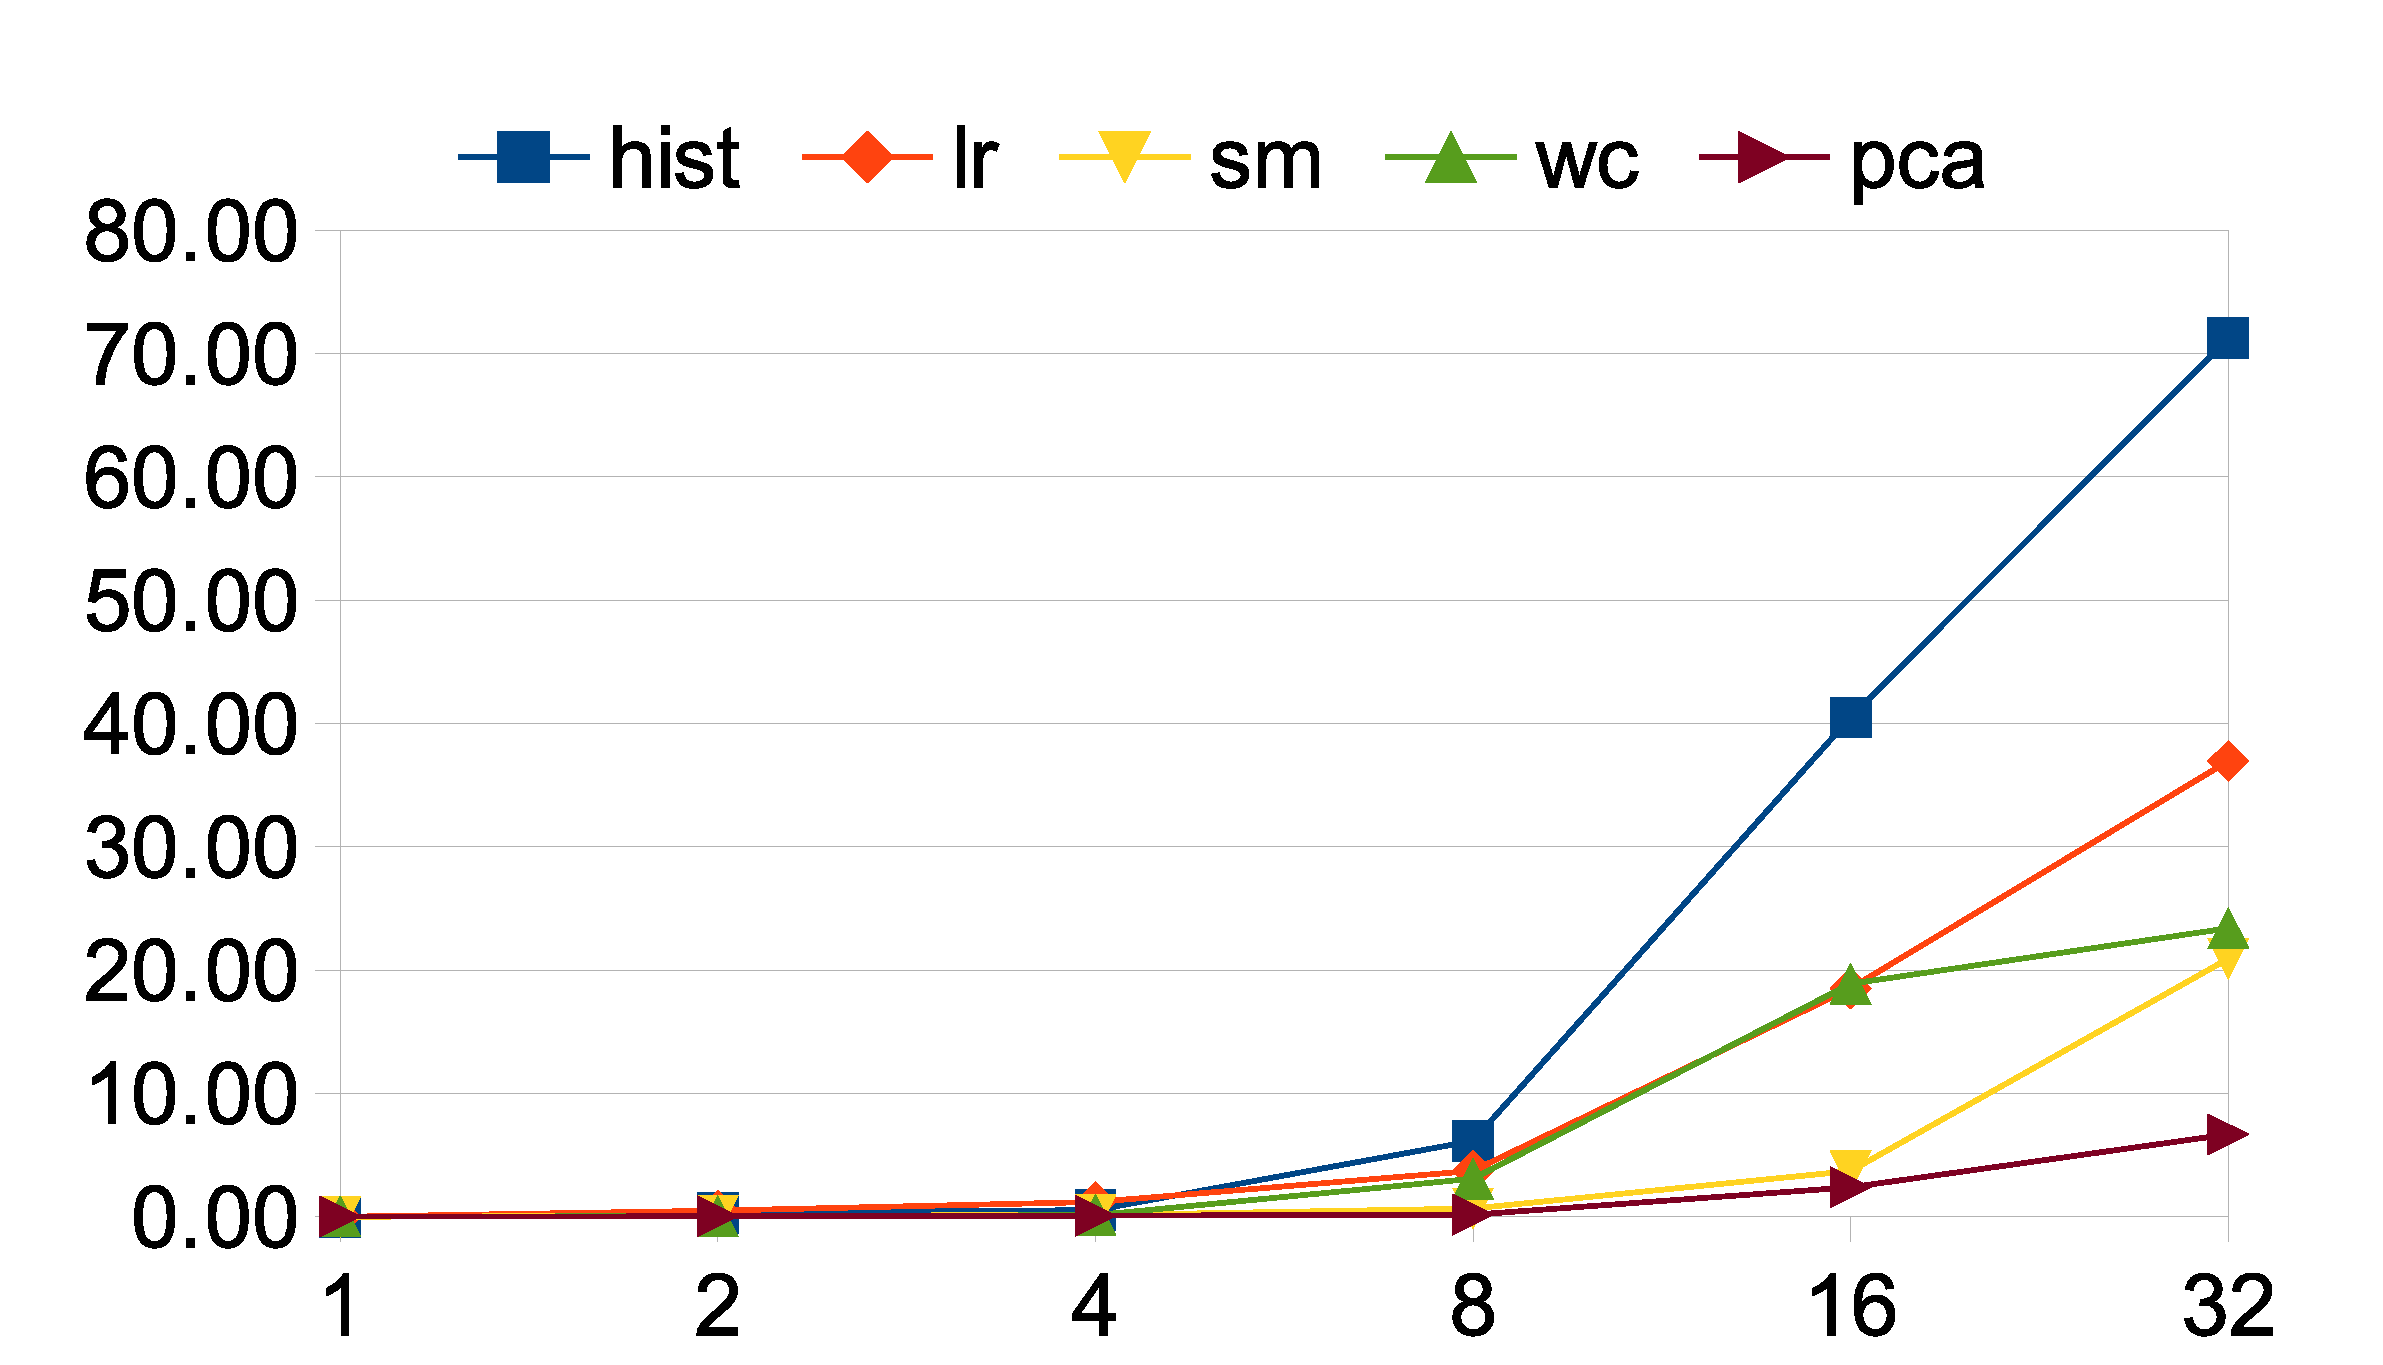
\includegraphics[width=0.5\textwidth]{img/phoenix_spinlock.eps}
    \caption{Phoenix运行过程中ticket\_spin\_lock所占百分比}
    \label{phoenix:spinlock}
\end{figure}

DMR将不再采用Pthreads线程模型,而是使用进程。
即每个map worker或reduce worker都是一个独立的进程。
由于进程拥有自己独立的地址空间,
拥有自己私有的mm\_sem,
由于不需要与其他进程共享信号量,
因此不存在锁的等待问题。
这可以避免上述多个线程竞争读写信号量导致的scalability问题。
然而,采用进程会带来一定的开销和不便,
主要表现在两方面:
(1)相比线程,创建进程的开销比较大。
(2)线程是基于共享内存的,因此线程间的数据的共享较简单,
而进程之间的共享需要一定的手段,
DMR中我们采用内存映射和隐式queue的方式,
用于map worker和reduce worker之间数据的传递。
进程的创建以及内存映射的环境构建,
都在DMR的初始化部分完成。
实验部分我们会详细分析DMR初始化的开销问题。

\subsubsection{通道的特征}
%无边界的通道
